\newcommand*\cols{2}
\newcommand*\rows{2}
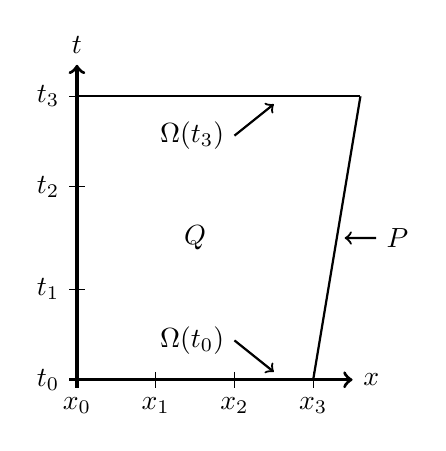
\begin{tikzpicture}[
    scale=1,
    axis/.style={very thick, ->},
    important line/.style={thick},
    every node/.style={color=black}
    ]
    %x-axis
    \draw[axis] (-0.1,0)  -- (3.5,0) node(xline)[right]{$x$};
    \foreach \x in {0,1,2,3}
    \draw (\x cm,0.1) -- (\x cm,-0.1) node[anchor=north] {$x_{\x}$};
    % t-axis
%    \draw[very thick] (0,-0.1) -- (0,1);
%    \draw[very thick] (0,1.3) -- (0,2.3);
    \draw[axis] (0,-0.1) -- (0,4) node(yline)[above]{$t$};
    \draw (0.1,0cm) -- (-0.1, 0cm) node[anchor=east] {$t_{0}$};
    \draw (0.1,1.15cm) -- (-0.1, 1.15cm) node[anchor=east] {$t_{1}$};
    \draw (0.1,2.45cm) -- (-0.1, 2.45cm) node[anchor=east] {$t_{2}$};
    \draw (0.1,3.6cm) -- (-0.1, 3.6cm) node[anchor=east] {$t_{3}$};
    % Lines
    \draw[important line] (3,0) coordinate (A)  -- (3.6,3.6) coordinate (B);
    \draw[important line] (0,3.6) coordinate (A)  -- (3.6,3.6) coordinate (B);
    \node (Q) at (1.5,1.8) {$Q$};
    \draw[thick,<-] (3.4,1.8cm) -- (3.8, 1.8) node[anchor=west] {$P$};
    \draw[thick,<-] (2.5,0.1cm) -- (2.0, 0.5) node[anchor=east] {$\Omega(t_0)$};
    \draw[thick,<-] (2.5,3.5cm) -- (2.0, 3.1) node[anchor=east] {$\Omega(t_3)$};
\end{tikzpicture}
